\begin{figure}
  \centering

  \begin{subfigure}{\textwidth}
    \begin{minipage}{0.7\textwidth}
      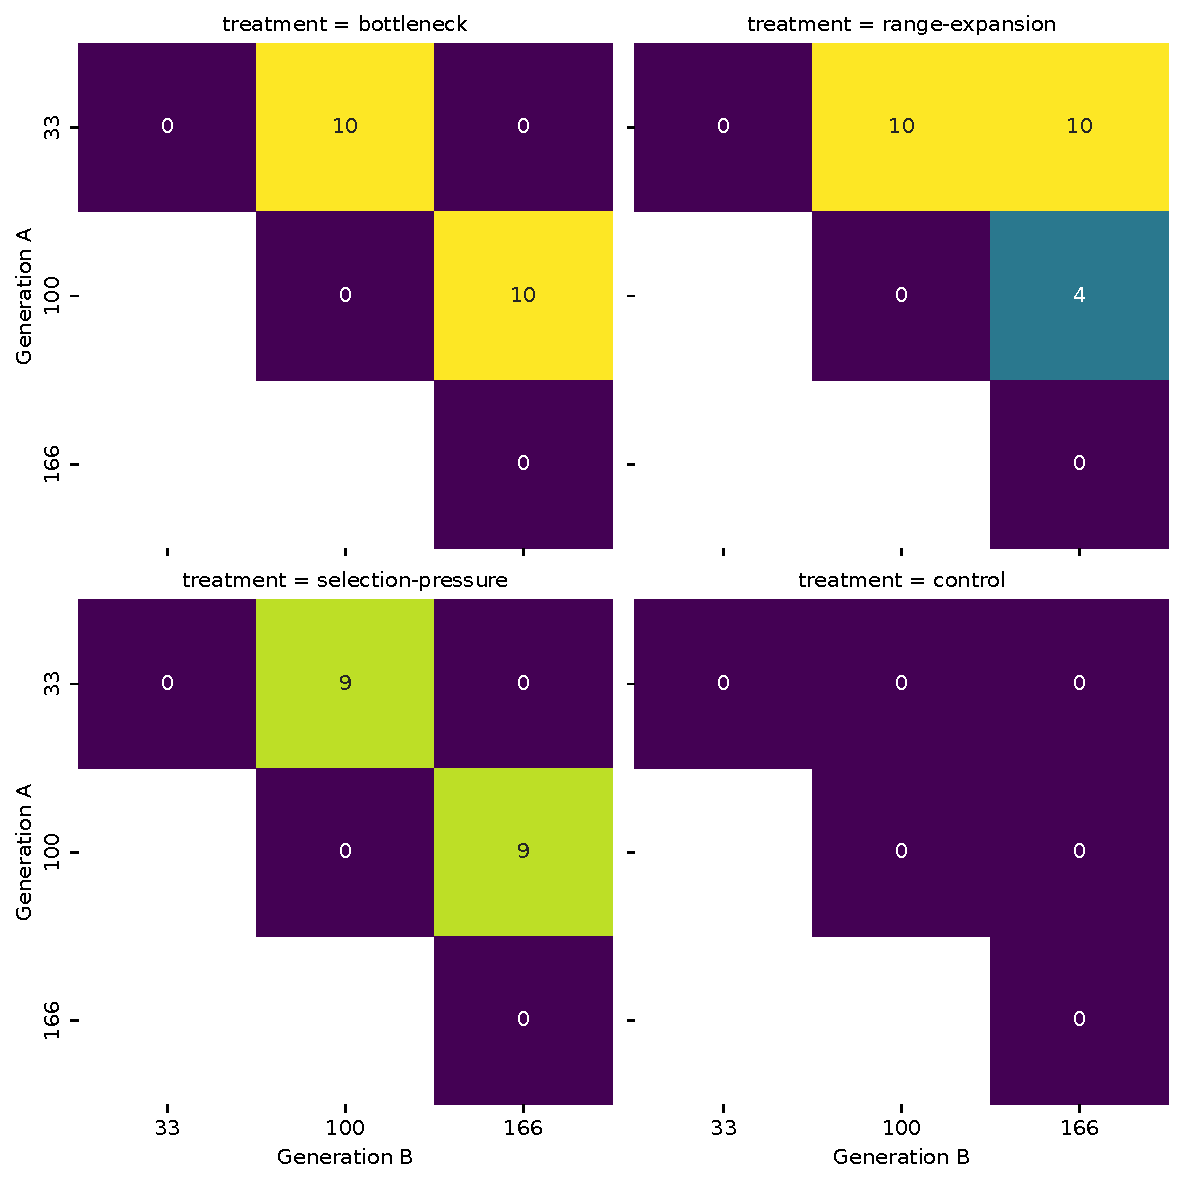
\includegraphics[width=\linewidth]{notebooks/notebooks/teeplots/hue=mann-whitney-significant-at-alpha-0-01+viz=facet-heatmap+x=generation-b+y=generation-a+ext=}
    \end{minipage}%
    \begin{minipage}{0.25\textwidth}
      \caption{Mann-Whitney comparison of 30 annotations at generations surrounding each target generation, with significance threshold $\alpha = 0.01$.}
      \label{fig:ne-detection-matrix:mann-whitney}
    \end{minipage}
  \end{subfigure}

  \vspace{1em} % adjust the vertical spacing between the subfigures

  \begin{subfigure}{\textwidth}
    \begin{minipage}{0.7\textwidth}
      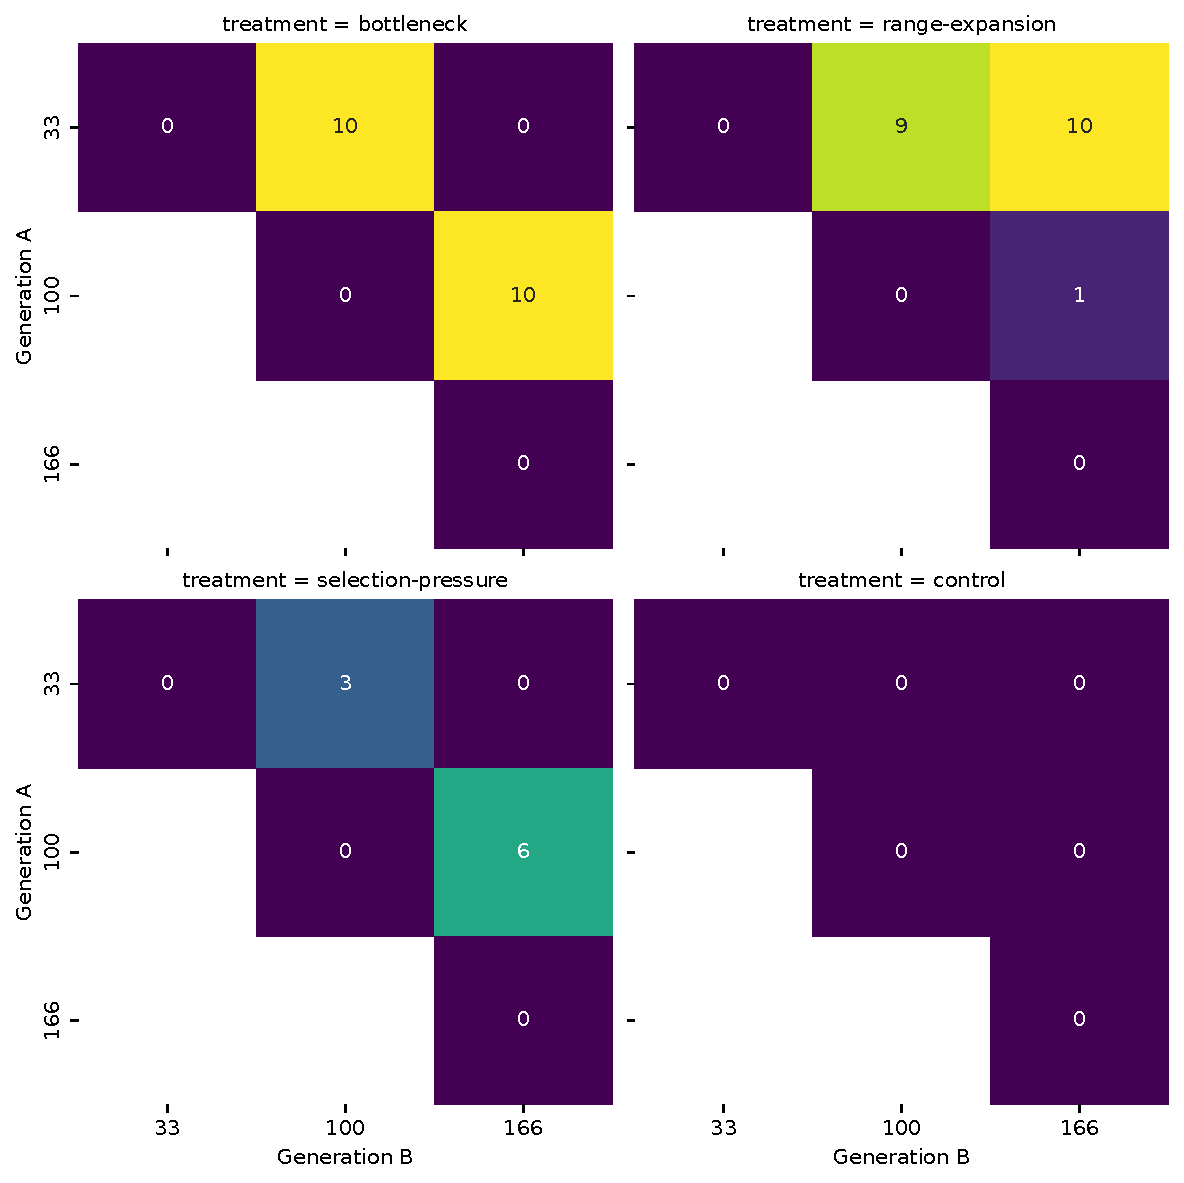
\includegraphics[width=\linewidth]{notebooks/notebooks/teeplots/hue=nonoverlapping-ci+viz=facet-heatmap+x=generation-b+y=generation-a+ext=}
    \end{minipage}%
    \begin{minipage}{0.25\textwidth}
      \caption{Non-overlapping MLE 95\% confidence intervals for rolling 10-sample estimate at target generations.}
      \label{fig:ne-detection-matrix:ci}
    \end{minipage}
  \end{subfigure}

  \caption{Counts of replicates where significant differences in effective population size ($N_e$) were detected between generation pairs.
  Counts are out of 10 total replicates attempted.
  All generation pairs had true differences in $N_e$, except same-generation pairs and generation pairs in the control experiment (Section \ref{sec:population-size-inference}).
  }
  \label{fig:ne-detection-matrix}
\end{figure}

% notebooks/notebooks/teeplots/hue=mann-whitney-significant-at-alpha-0-01+viz=facet-heatmap+x=generation-b+y=generation-a+ext=.pdf
%
% notebooks/notebooks/teeplots/hue=nonoverlapping-ci+viz=facet-heatmap+x=generation-b+y=generation-a+ext=.pdf
